\chapter{Background}

\section{Chernoff's 2-player game}
Tbd whether relevant.

\section{Bandits}
%What is the scenario/model?
The so-called stochastic multi-armed bandits is a general model to simulate decision-making in uncertain environments.
In particular, one assumes a set of options or arms to choose from, each choice leading to an outcome, also referred to as reward. In general, one assumes many sequential selections among the set of arms. It is typically assumed that the outcome of the selection of an individual arm follows a fixed but unknown probability distribution.

%What problems are typically tackled by this scenario?
Within the bandits model, the concern revolves around which arm to choose next. Allocation strategies tackling this question address either of two problems: explore-exploit or pure-explore.

The former concerns itself with maximizing the \emph{cummulative reward}. This means that one attempts to maximize the \emph{sum of the rewards obtained} through all arm selections. Naturally, starting off without any knowledge about the underlying distributions, this involves both exploration of arm qualities as well as exploitation of gathered knowledge.

The latter revolves around \emph{simple reward}. This problem consists of seeking to maximize the reward one obtains if one leverages the current knowledge for \emph{another} draw. This implies that the focus lies on \emph{identification} of high-quality candidates, where quality is usually assessed by high means. Hence it is part of the task to make estimated best and true best equal as well as obtaining a high \emph{confidence} on this statement.

%Why is model and its problems relevant?
The bandits model can be used for all processes involving sequential decision making. Yet, an important simplification is the assumption of the distributions being fixed over time. This assumption might be more or less representative of the true, to-be-modelled processes.

The explore-exploit problem is applied in Recommender Systems, ad campaigns, in the context of Reinforcement Learning and Robotics.

For real-world applications of the pure-exploration bandit please refer to \ref{ss:top-1_model}.

There exist many specialized versions of the Bandits model, such as contextual bandits or adversarial bandits.

\section{Thompson Sampling}
%How does it work?
%Why is it useful?
%What is it used for?

Thompson sampling is a sampling strategy often employed for choosing arms in the bandits scenario. By default, it particularly lends itself to the cummulative reward setting. The technique is based on having and updating prior distributions over all arms. In contrast to greedily selecting the arm that empirically maximizes the metric of desire, Thompson sampling suggests to randomly draw beliefs on arms from the prior distributions. Subsequently, it selects the arm which maximizes the metric of desire on the sampled belief.
With many repetitions, this leads to each arm being sampled proportionally to its likelihood of maximizing the metric of desire according to current belief.
Intuitively, this is very appealing for the cummulative reward scenario as it creates a natural balance between exploration and exploitation.

% Insert algorithm from overview paper?

\section{Notation}
We assume $k$ arms to choose from and denote the set of possible arms as $[k]$. Subsets $S \subset [k]$ are assumed to be of size $m < k$.

A possible set of means for the arms is denoted as the $k$-dimensional vector $\theta$, where every mean can lie between 0 and 1. We also refer to such a $\theta$ as parameter.

Finding ourselves in a frequentist setting, we assume an underlying true mean of the arms refer to this as $\theta^*$. Moreover, this ground truth implies a true best arm $l^*$ and true top-$m$ arms $S^*$. When referring to an individual arm in the top-$m$ case, we proceed to use $j$ for arms in $S^*$, $i$ for arms not in $S^*$ and $l$ for arms of which this knowledge does not exist.

Given the constraint that the means lie between 0 and 1, there are infinitely many possible parameter vectors which make arm $l \in [k]$ the best one under $\theta$ or $S \subset [k]$ top-$m$ under $\theta$. Hence we group such $\theta$ in the following way:
\begin{align}
  \Theta &:= [0, 1]^k \\
  \Theta_{1, l} &:= \{\theta \in \Theta | l = \argmax_{l' \in [k]} \theta_{l'}\} \\
  \Theta_{m, S} &:= \{\theta \in \Theta | S = \text{top-}m(\theta)\} \\
    &= \{ \theta \in \Theta| \min_{j_1 \in S}\ \theta_{j_1} > \max_{j_2 \notin S}\ \theta_{j_2}\} \\
  \Theta_{m, l} &= \{\theta \in \Theta | l \in \text{ top-}m(\theta)\}
\end{align}
where top-$m$ returns the $m$ highest values, i.e. means, from its argument $\theta$.

After having made $n$ observations of rewards, bundled in $D_n$, $\Pi_n$ expresses a posterior distribution with density $\pi_n$ over elements of $\Theta$. E.g. for sets $\Theta_{m, S}$, we have:
\begin{align}
  \Pi_n(\Theta_{m, S}) &:= \int_{\theta \in \Theta_{m, S}} \pi_n(\theta) d\theta \\
    &= \Pr[S \text{ is top-}m | D_n]
\end{align}
Clearly, it holds that $\Pi_n(\Theta) = 1$. As a shorthand for the top-$m$ case, we will use:
\begin{align}
  \alpha_{n, l} &:= \Pi_n(\Theta_{m, l}) \\
  \alpha_{n, S} &:= \Pi_n(\Theta_{m, S})
\end{align}
We are mostly interested in strategies that allocate measurement effort over the arms in a randomized fashion, i.e. according to a probability distribution. We refer to such an allocation or distribution as $\psi$, defining the probability of each arm being sampled. Naturally, it holds that $\sum_{l \in [k]} \psi_l = 1$.

The $n$-th sampled arm is denoted as $l_n$. For adaptive strategies, the allocation can change after every sample. After $n$ sample we refer to the allocation s as $\psi_{n}$ and therefore after $n$ samples we have $\psi_{n, l} = \Pr[l_n = l]$ for arm $l$. We also define the allocation property of a set by the sum of its arms: $\psi_S = \sum_{l \in S} \psi_l$. In the case of adaptive strategies, we might as well be interested in average allocation up to a certain sample $n$. We write:
\begin{align}
  \bar{\psi}_{n, l} &:= \frac{\sum_{n' = 1}^{n} \psi_{n', l}}{n}
\end{align}
We use the notation $d(\theta_1||\theta_2)$ to represent the Kullback-Leibler divergence between $\theta_1$ and $\theta_2$.

\section{Best Arm Identification}
\subsection{Model}\label{ss:top-1_model}
%What is the problem?
%Why is it relevant?
%How is performance evaluated? What is 'confidence'?

Best Arm identification implies disregarding the sum of the rewards encountered while sampling. Rather, the goal is to efficiently gather information maximizing the confidence of the suggestion made \emph{after} the sampling phase. In other words, there is a purely explorative phase, also referred to as 'experiment' which is then typically followed by a purely exploitative phase, having committed to an option. For this reason, Best Arm Identification is also known as 'Experiment Design'.

Quite naturally, all other aspects being controlled for, requiring fewer samples is preferable. Hence one can formulate the goal in two ways: maximize confidence for a fix amount of samples or minimize amount of samples for a fixed confidence.

Confidence can mean and be evaluated in different ways. For Bayesian algorithms, it is possible to quantify the confidence the model has in the currently most favourable looking candidate. This quantity corresponds to the mass a posterior puts on parameters favouring said candidate. Another approach to measure confidence stems from the realm of Probably approximately correct learning, or PAC in short. In the PAC context, one desires to make a statement of the sort $\Pr[\text{output of algoritm is $\epsilon$-correct}] \geq 1 - \delta$, where $\epsilon$-correctness requires an explicit definition. In this case, under the toleration of $\epsilon$, $1 - \delta$ can be thought of as confidence.

Real-world applications of Best Arm identification include:
\begin{itemize}
  \item Physical simulations: Given a collection of designs, e.g. the bodywork of a car, determine e.g. aerodynamic properties of the cars. Elaborate simulations can come with significant resource demands, such as compute power and direct and indirect costs of losing time. Coming to the same conclusion, consisting of the superiority of one of the designs, with fewer simulations can be crucial.
  \item Crop selection: Experimenting different crop types in a given growing environment measuring yields, generate a recommendation for that same growing environment.
\end{itemize}

"ML: drive generation of own data instead of" -> it is about acquisition

\subsection{Optimal allocation}\label{subsection:optimal_allocation}
% TODO: explain limiting assumptions made by Russo

% What is the overall goal?
% How is this achieved? (Talk about optimization over hyper-parameters)

We start off by describing what it means for an allocation to be optimal and by enumerating some of its properties. We do not present a constructive allocation, rather we assume knowledge about the underlying truth to provide a best possible bound. Intuitively it is not possible to match the performance of that optimal allocation without the knowledge of the underlying truth. Hence the desired statement is to say that a concrete adative allocation \emph{converges} to the optimal allocation.

As mentioned in \ref{ss:top-1_model}, the goal consists of maximizing confidence, i.e. the mass the posterior lays onto the true best arm. Oberve that for any allocation sampling each arm infinitely many times, this quantity will tend towards 1. What makes the optimal allocation optimal is the rate at which the posterior of the true arm convergence towards 1.

Note that the optimal allocation assumes knowledge about the underlying true value and therefore does not need to be adaptive. It can be framed as the following thought experiment: Assume you know the true underlying means. Yet your adversary doesn't trust your 'knowledge'. He only trusts the sample rewards that he can observe for himself. Now it is your task to leverage your knowledge about the true means to sample most the arms in a way that convinces the adversary as quickly as possible.

\subsubsection{Rate of convergence}
Russo \cite{DBLP:journals/corr/Russo16} shows that the rate at which the posterior $\Pi_n$ of the set parameters under which the true best arm $l^*$ is optimal $\Theta^*$ cannot be faster than the following:
\begin{align}
  \Pi_n(\Theta_{l^*}) &= 1 - \Pi_n(\Theta^c_{l^*}) = 1 - \exp\{-n\Gamma^*\} \\
  \Gamma^* &= \max_{\psi} \min_{\theta \in \Theta^c_{l^*}} \sum_{l \in [k]} \psi_l d(\theta_l^* || \theta_l)
\end{align}
where $n$ corresponds to the number of samples acquired.

The allocation $\psi$ maximizing this quantity is what we refer to as optimal allocation.

\subsubsection{Defining properties}
Russo's underlying idea is that the optimal allocation gathers equal \emph{evidence}, e.g. compared to having equal effort for a uniform distribution. This notion of evidence relies on the comparison between the true best against all other arms. It takes both their respective true means as well as sampling frequencies into consideration. For an allocation $\psi$, he defines
\begin{align}
  C_i(\psi_{l^*}, \psi_i) := \min_{x \in \mathbb{R}} \psi_{l^*} d(\theta_{l^*}^*||x) + \psi_i d(\theta_{i}^*||x)
\end{align}
and goes on to show that the optimal allocation $\psi^*$ is identified by fulfilling the condition
\begin{align}
  \forall i_1, i_2 \neq l^*: C_{i_1}(\psi_{l^*}, \psi_{i_1}) = C_{i_2}(\psi_{l^*}, \psi_{i_2})
\end{align}
Moreover, he shows that the optimal allocation is unique.

\subsection{A Constrained Optimal Allocation}
%What are properties of the constrained optimal allocation?
%How can they be interpreted?

In order to bridge the gap between algorithm and optimal allocation, Russo introduces the concept of \emph{constraining} the optimal allocation. His algorithm naturally implies the constraint that in the limit, $\beta$ of the measurement effort is allocated to the true best arm.

He is able to show that his algorithm's allocation converges to the overall optimal allocation by showing that
\begin{itemize}
  \item The algorithm's average allocation $\bar{\psi}_n$ converges to the optimal allocation under the constraint $\psi_{l^*}^* = \beta$
  \item The hyperparameter $\beta$ can be tuned to equal the overall optimal value.
\end{itemize}
The optimal convergence exponent under said constraint becomes:
\begin{align}
  \Gamma^*_{\beta} &= \max_{\psi: \psi_{l^*} = \beta} \min_{\theta \in \Theta^c_{l^*}} \sum_{l \in [k]} \psi_l d(\theta_l^* || \theta_l)
\end{align}

\subsection{Top-Two Thompson Sampling algorithm}
% What is the algorithm?

Russo proposes different algorithms that satisfy aforementioned theoretical results, yet suggests that one of them outperfoms the other empirically: Top-Two Thompson Sampling (TTTS) algorithm.

The main idea behind TTTS \ref{alg:TTTS} is to repeat drawing with Thompson sampling from the prior until two different candidates are obtained. This illustrates how Thompson sampling, usually only truly useful for exploit-explore settings can be used for pure-exploit: some of its focus is shifted towards inferior-looking candidates. Among those two candidates, the former is picked with probability $\beta$, explaining the provenance of the hyperparameter.

% TODO: Pi prior or posterior?
\begin{algorithm}[H]
    \caption{Given a prior $\Pi_n$ at step $n$}
    \label{alg:TTTS}
  \begin{algorithmic}
    \State $\hat{\theta} \sim \Pi_n$
    \State $l_1 := \argmax(\hat{\theta})$
    \Repeat
      \State $\hat{\theta} \sim \Pi_n$
      \State $l_2 := \argmax(\hat{\theta})$
    \Until{$l_1 \neq l_2$}
    \State $B \sim Bernoulli(\beta)$
    \If{$B=1$}
      \State $l_n := l_1$
    \Else
      \State $l_n := l_2$
    \EndIf
    \State Play $l_n$, observe reward and update priors
  \end{algorithmic}
\end{algorithm}

The attentive reader might wonder how exactly prior/posteriors are updated. This is addressed in the empirical section \ref{section:empirical_behaviour}.

\subsection{Alternative approaches}
What are alternative approaches to Russo's?
How do they compare against Russo's?

\section{Top-$m$ Arm Identification}
% What is the problem?
% Why is it relevant compared to Top-1?

Top-$m$ Arm Identification is a generalization of Best Arm Identification. The objective is to identify the set of arms, with cardinality $m$, which contains the $m$ best arms.

Applications of top-$m$ arm identification are similary to those mentioned in \ref{ss:top-1_model}. Natural explications for desiring the identification $m$ instead of 1 high-quality option can be diversification or regulation.

\subsection{Current approaches: LUCB}
How are those methods evaluated?
What are possible qualitative shortcomings of those methods?
What are possible quantitative shortcomings of those methods?

The general LUCB algorihm can be seen in \ref{alg:LUCB1}. For every arm $l$, an empirical mean $\hat{\mu}_l^t$ is kept and updated after each sample. The overall idea is to compute a confidence bound for every arm, in every step. Per round, arms are separated into two sets: the arms with the $m$ best empirical means, $Top(t)$ and the rest, $Bottom(t)$. The arm with the lowest lower confidence bound from $Top(t)$ and the arm with the hightest upper confidence bound from $Bottom(t)$ are sampled and all information updated.
The algorithm stops once its stopping criterion is met. The confidence bound of an arm $l$ equals $(\hat{\mu}_l^t - \beta(l), \hat{\mu}_l^t + \beta(l))$.
Kalyanakrishnan et al. \cite{DBLP:conf/icml/KalyanakrishnanTAS12} propose a concrete instantiation:
\[\beta(l) = \]

\begin{algorithm}[H]
    \caption{Given a prior $\Pi_n$ at step $n$}
    \label{alg:LUCB1}
  \begin{algorithmic}
    \State Play $l_n$, observe reward and update priors
    \State Sample each arm once
    \Repeat
      \State Compute $Top(t), Bottom(t), h_*^t, l_*^t$
      \State Sample $h_*^t$ and $l_*^t$
      \State Update $\hat{\mu}_t$ and confidence bounds
    \Until{$ \mu < \epsilon$}
  \end{algorithmic}
\end{algorithm}


\subsubsection{Confidence estimation 1}
\subsubsection{Confidence estimation 2}
\subsubsection{Confidence estimation 3}


\chapter{Charactarizing the Constrained Optimal Top-$m$ Allocation}

%TODO: Talk about prior vs posterior.
%TODO Talk about limitations on distributions.
%What does it mean to be optimal?
Analogously to \ref{subsection:optimal_allocation}, we define the optimal top-$m$ allocation by its convergence rate of the posterior mass put on parameters reflecting the true top-$m$ arms $\Pi_n(\Theta_{m, S^*})$. Moreover, just as in Russo's top-1 case, the algorithm we will propose introduces a constraint. We will also put the optimal allocation under that constraint with the idea being that this is but a hyperparameter that can be optimized over.

In \Cref{section:optimal_statements} we first introduce some of Russo's results that also apply in our scenario. Then we will introduce some general properties, followed by a complete characterization of the optimal allocation. Proofs of the statements are provided in \Cref{section:optimal_proofs}. Moreover, we will show an example of a concrete optimal allocation in \Cref{section:conrete_optimal_allocation}.

Overall we hope to convince the reader that the chracterization results portrayed in this chapter make for a natrual generalization of Russo's top-1 case. The guiding theme will be that instead of comparing the best arm $l^*$ to a suboptimal arm that is the hardest to distinguish from it, we will compare the a pair of an optimal and a suboptimal arm are hardest to distinguish from another. Note that again, distinction revolves around two factors: the frequency with which an arm has been sampled, i.e. quantity, as well as the proximity of its true mean, i.e. quality.

%%%%%%
% Statements
%How can C be interpreted?
%How does this tie in with Chernoff's statements?
%How does this compare to the top-1 case?
%What's an example of an optimal allocation?
%How would those statements look like without the constraint?
%%%%%

\section{Statements}\label{section:optimal_statements}
Russo proves a proposition about the posterior convergence rate about general parameter sets $\tilde{\Theta}$.

\begin{proposition}[Russo: Proposition 5]\label{proposition:prop5}
  For any open set $\tilde{\Theta} \subset \Theta$ and average allocation $\bar{\psi}_n$
  \[\Pi_n(\tilde{\Theta}) \deq \exp\{-n \inf_{\theta \in \tilde{\Theta}} \sum_{l \in [k]} \bar{\psi}_{n, l} d(\theta^*_l || \theta_l)\}\]
\end{proposition}

As mentioned before, we seek to analyze how fast $\Theta_{S^*}$ converges to 1. Clearly we have $\Theta_{S^*} = 1 - \Theta_{S^*}^c$. Hence instead of analyzing the rate of convergence of $\Pi_n(\Theta_{S^*})$ to 1, we can analyze the rate of convergence of $\Pi(\Theta_{S^*}^c)$ to 0.

Instead of analyzing $\Pi_n(\Theta_{m, S^*}^c)$ directly, we express it with via $\Theta_{m, l}$ and its relaxation $\tilde{\Theta}_i$. Intuitively, $\bar{\Theta}_i$ is the set of parameters under which $i$ proves that $S^*$ is not optimal.
\begin{align}
    \bar{\Theta}_i &= \{ \theta \in \Theta | \text{top-}m(\theta, S^* \cup \{i\}) \neq S^*\}
\end{align}
Observe that we have $\bar{\Theta}_i \supsetneq \Theta_i$. Moreover we present a useful relationship between $\Theta_{m, S^*}^c$ and $\bar{\Theta}_i$:
\begin{lemma}\label{lemma:set_relation_S*_i}
  \[\Theta_{m, S^*}^c = \bigcup_{i \notin S^*} \bar{\Theta}_i\]
\end{lemma}
Leveraging this relationship of the sets allows us to bridge the gap between the posterior of $\Theta_{m, S^*}^c$ and the posterior of individual sets $\bar{\Theta}_i$. Note the transition from a union of sets to a minimum over sets permitted by the usage of the $\deq$ equality, as shown in \Cref{lemma:posterior_S*_i}.
\begin{lemma}\label{lemma:posterior_S*_i} If $\alpha_{n, S^*} \rightarrow 1$, then
  \begin{align}
    \Pi_n(\Theta_{m, S^*}^c) \deq \max_{i \notin S^*} \Pi_n(\bar{\Theta}_i) \deq 1 - \min_{j \in S^*} \Pi_n(\Theta_j)
  \end{align}
\end{lemma}

Plugging $\bar{\Theta}_i$ into \ref{proposition:prop5} leaves us with a sum of KL divergences. We seek to simplify this sum to individual terms just after defining:
\begin{align}
  C_{j, i}(\psi_j,\psi_i) &=  \min_{x \in \mathbb{R}} \psi_j d(\theta^*_{j} || x) + \psi_i d(\theta_{i}^* ||x) \label{eq:C}
\end{align}
% TODO: Talk about player scenario?
In particular, $C_{j, i}$ can be thought of as evidence that $j$ is distinct from $i$. Quite naturally, we want this evidence as large as possible for every pair $(j, i) \in S^* \times {S^*}^c$.

\begin{lemma}\label{lemma:kl_to_C}
  For any $i \notin S^*$ and any allocation $\psi$,
  \begin{align}
    \min_{\theta \in \bar{\Theta}_i} \sum_{l \in [k]}\psi_l d(\theta^*_l||\theta_l) = \min_{j \in S^*} C_{j, i}(\psi_j, \psi_i)
  \end{align}
\end{lemma}

Intuitively, this lemma tells us that the weighted sum of KL divergences can be reduced to looking at only two arms for parameters in $\Bar{\Theta}_i$. One of those arms will be $i$. The other has arm to stem from the true set of arms $S^*$ in order to satisfy $\Bar{\Theta}_i$'s requirement of 'disproving' $S^*$. This arm $j \in S^*$ is chosen as to seem the 'least distinctive' from i. Distinction is made up of two aspects, as seen in the definition of $C_{j, i}$ in \eqref{eq:C}: how much this arm $j$ is sampled, i.e. $\psi_j$, and how different its true mean is from the true mean of j, captured by the KL divergence between both arms and an $x$ inbetween, individually.

We can apply those statements to the quantity we care about: the mass the posterior puts on the complement of parameters reflecting the true top-$m$ arms $\Theta_{S^*}^c$.

For a given allocation $\psi$, we have:
\begin{align}
  \Pi_n(\Theta_{S^*}^c) &\deq \max_{i \notin S^*}\Pi_n(\hat{\Theta}_i) \text{ (\Cref{lemma:posterior_S*_i})}\\
    &\deq \max_{i \notin S^*} \exp\{-n\inf_{\theta \in \hat{\Theta}_i} \sum_{l \in [k]} \bar{\psi}_{n, l} d(\theta^*_l || \theta_l)\} \text{ (\Cref{proposition:prop5})} \\
    &= \max_{i \notin S^*} \exp\{-n \min_{j \in S^*} C_{j, i}(\psi_j, \psi_i)\} \text{ (\Cref{lemma:kl_to_C})} \\
    &= \exp\{-n \min_{i \notin S^*}\min_{j \in S^*} C_{j, i}(\psi_j, \psi_i)\} \label{eq:posterior}
\end{align}
In other words, the rate at which the posterior converges to the truth with increasing number of samples is defined by the pair of optimal and suboptimal arms for which the least evidence exists.

As we've described, the optimal allocation $\psi^*$ is the one which makes the quantity from \eqref{eq:posterior} as small as possible. We have:
\begin{align}
  \psi^* &= \argmin_{\psi} \exp\{-n \min_{i \notin S^*}\min_{j \in S^*} C_{j, i}(\psi_j, \psi_i)\} \\
    &= \argmax_{\psi} \min_{i \notin S^*}\min_{j \in S^*} C_{j, i}(\psi_j, \psi_i) \label{eq:psi^*}
\end{align}
For the sake of convenience we define the optimal exponent:
\begin{align}
  \Gamma^* = \max_{\psi} \min_{i \notin S^*}\min_{j \in S^*} C_{j, i}(\psi_j, \psi_i) \label{eq:gamma^*}
\end{align}

\paragraph{An Optimal Constrained Allocation}

%TODO: Talk about being able to do with j what we did through \theta_i.

Our proposed algorithm will always allocate $\frac{1}{2}$ of its samples to arms in $S^*$ in the long run. As a consequence it may not attain the overall optimal exponent without hyperparameter tuning. Hence we consider a modified, constrained setting under which the algorithm performs optimally. By adapting \eqref{eq:psi^*} and \eqref{eq:gamma^*} we obtain:
\begin{align}
  \psi^{\frac{1}{2}*} &= \argmax_{\psi: \psi_{S^*}=\frac{1}{2}} \min_{i \notin S^*}\min_{j \in S^*} C_{j, i}(\psi_j, \psi_i) \label{eq:constrained_optimal_psi}\\
  \Gamma^{\frac{1}{2}*} &= \max_{\psi, \psi_{S^*} = \frac{1}{2}} \min_{i \notin S^*} \min_{j \in S^*} C_{j, i}(\psi_j, \psi_i) \label{eq:constrained_optimal_gamma}
\end{align}
Hence we have established the optimal constrained rate of convergence $\Gamma^{\frac{1}{2}*}$ of the optimal constrained allocation $\psi^{\frac{1}{2}*}$ by making a link to the minimization over $C_{j, i}$ . We seek to further characterize $\psi^{\frac{1}{2}*}$ by relying on the same maxim as in Russo's scenario: we expect the measurement plan to collect \emph{equal evidence}, not \emph{equal measurement} for every arm. Hence in \Cref{proposition:characterization} we will show that the optimal measurement plan will fulfill \eqref{eq:condition_C}. Before doing so, we set the stage by enounciating two properties of $C_{j, i}$.

\begin{lemma}\label{lemma:C_concave}
  Each $\min_{j \in S^*} C_{j, i}(\psi_j, \psi_i)$ is a concave function.
\end{lemma}

\begin{lemma}\label{lemma:C_unique_solution}
  Given a $j \in S^*$, the solution to the minimization problem \eqref{eq:C} in $x$ is $\bar{\theta} \in \mathbb{R}$, satisfying:
  \[A'(\bar{\theta}) = \frac{\psi_j A'(\theta_j^*) + \psi_i A'(\theta_i^*)}{\psi_j + \psi_i}\]
  where $A'(\theta)$ is the mean observation under $\theta$. Therefore
  \[\min_{j \in S^*} C_{j, i}(\psi_j, \psi_i) = \min_{j \in S^*} \psi_j d(\theta^*_j || \bar{\theta}) + \psi_i d(\theta^*_i || \bar{\theta})\]
\end{lemma}

\begin{proposition}\label{proposition:characterization}
  The solution to the optimzation problem \ref{eq:constrained_optimal_psi} is the allocation $\psi^{\frac{1}{2}*}$, which is unique and satisfies
  \begin{align}
    \forall j_1, j_2 \in S^*, \forall i_1, i_2 \notin S^*: C_{j, i}(\psi^*_{j_1}, \psi^*_{i_1}) = C_{j, i}(\psi^*_{j_2}, \psi^*_{i_2})\label{eq:condition_C}
  \end{align}
  If $\psi_n = \psi^*$ for all $n$, then
  \[\Pi_n(\Theta_{S^*}^c) \deq \exp \{-n\Gamma^*_{\frac{1}{2}}\}.\]
  Moreover, under any other adaptive allocation rule, if $\bar{\psi}_{n, S^*} \rightarrow \frac{1}{2}$ then
  \[\lim_{n \rightarrow \infty} \sup - \frac{1}{n} \log \Pi_n(\Theta^c_{S^*}) \leq \Gamma^*_{\frac{1}{2}}\]
  almost surely.
\end{proposition}

\section{A Concrete Optimal Allocation}\label{section:conrete_optimal_allocation}
For the sake of concreteness, we present numeric values of optimal allocations, both constrained and unconstrained for two top-$m$ identification scenarios.
Hence given, the true means $\theta^*$, we seek to determine $\psi^*$ and $\psi^{\frac{1}{2}*}$. Relying on \eqref{eq:condition_C}, we have a massively over-determined system of equations. The latter can be approximately solved by numerical methods, in our case least squares minimization.

For this concrete example, we assume arm rewards to follow Bernoulli distributions with means $\theta_1$ and $\theta_2$ respetively. Thanks to this assumption, the KL divergences can be minimized analytically with great convenience, we refer to the appendix, \Cref{section:bernoulli_c} for details. \Cref{fig:optimal_allocation} indicates the probaility mass put onto each arm for each scenario. The results were produced with for a top-4 scenario with
\begin{itemize}
  \item $\theta_1 = [.1,\ .2,\ .3,\ .4,\ .5,\ \underbrace{.6,\ .7,\ .8,\ .9}_\text{$S^*$}]$
  \item $\theta_2 = [.4,\ .425,\ .45,\ .475,\ .5,\ \underbrace{.525,\ .55,\ .575,\ .6}_\text{$S^*$}]$
\end{itemize}

Fur further details we refer to the simulation code in our repository \footnote{\url{https://github.com/kkleindev/ttts/compute_optimal_allocation.py}}.

\begin{figure}[h]
  \centering
  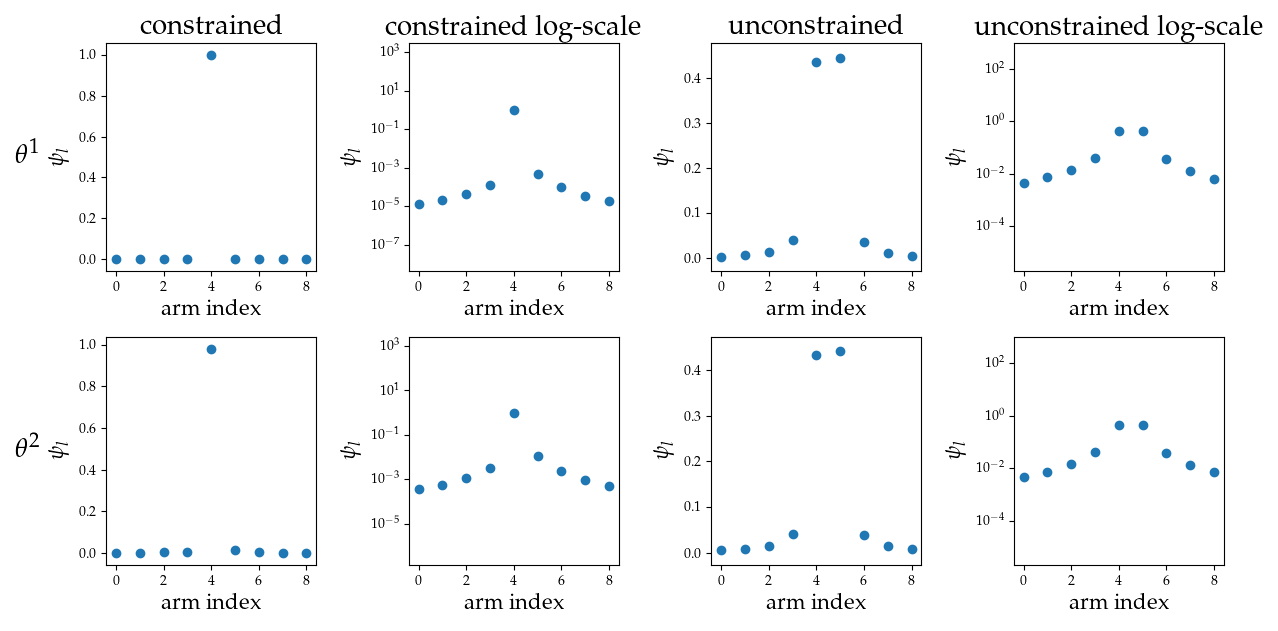
\includegraphics[width=\textwidth]{optimal_allocation.png}
  \caption{Unconstrained and constrained optimal allocation for $\theta_1$ and $\theta_2$, top-4}
  \label{fig:optimal_allocation}
\end{figure}

TODO: Propose an intuition why the concentration is so high in unconstrained scenario.

\section{Proofs}\label{section:optimal_proofs}
\begin{proof}[\Cref{lemma:set_relation_S*_i}]
  \begin{align}
    \Theta_{m, S^*}^c &= \{\theta \in \Theta | \min_{j \in S^*} \theta_j > \max_{i \notin S^*} \theta_i \}^c \\
    &= \{\theta \in \Theta | \max_{i \notin S^*} \theta_i \geq \min_{j \in S^*} \theta_j\} \\
    &= \{\theta \in \Theta | \exists i \notin S^*: \theta_i \geq \min_{j \in S^*} \theta_j\} \\
    &= \{\theta \in \Theta | \exists i \notin S^*: \text{top-}m(\theta, S^* \cup \{i\}) \neq S^*\} \\
    &= \bigcup_{i \notin S^*} \{\theta \in \Theta | \text{top-}m(\theta, S^* \cup \{i\}) \neq S^*\} \\
    &= \bigcup_{i \notin S^*} \bar{\Theta}_i
  \end{align}
\end{proof}

\begin{proof}[\Cref{lemma:posterior_S*_i}]
  \begin{align}
    \max_{i \notin S^*} \Pi_n(\bar{\Theta}_i) \leq \Pi_n(\Theta_{m, S^*}^c) \leq (k-m) \max_{i \notin S^*} \Pi_n(\bar{\Theta}_i)
  \end{align}
  This equation follows from \Cref{lemma:set_relation_S*_i} and the fact that the union has an additive effect with respect to the density $\Pi_n$. There are $k-m$ possible $i$s and each single one leads to a set, whose density is bounded by the maximal density of all such sets.
  Asymptotically this gives
  \begin{align}
    \Pi_n(\Theta_{m, S^*}^c) \deq \max_{i \notin S^*} \Pi_n(\bar{\Theta}_i)
  \end{align}
  For $S^*$, we have:
  \begin{align}
    &\Theta_{m, S^*}^c = \Theta - \bigcap_{j \in S^*} \Theta_j \\
    &1 - \min_{j \in S^*} \Pi(\Theta_j) \leq \Pi(\Theta_{m, S^*}^c) \leq 1 - \min_{j \in S^*} (\Pi(\Theta_j))^m \\
    &\lim_{n \rightarrow \infty} \frac{1}{n} \log(\frac{\min_{j \in S^*} \Pi(\Theta_j)}{\min_{j \in S^*} (\Pi(\Theta_j))^m}) = \lim_{n \rightarrow \infty} \frac{-(m - 1)}{n} \log(\min_{j \in S^*} \Pi(\Theta_j))
  \end{align}
  Observe that $\min_{j \in S^*} \Pi(\Theta_j) \geq \alpha_{n, S^*} \rightarrow 1$. Hence the limit of the fraction goes to 0 and we have $\min_{j \in S^*} \Pi(\Theta_j) \deq \min_{j \in S^*} (\Pi(\Theta_j))^m$. Again, by the Squeeze theorem it follows that
  \begin{align}
    \Pi_n(\Theta_{m, S^*}^c) \deq 1 - \min_{j \in S^*} \Pi_n(\Theta_j)
  \end{align}
\end{proof}

\begin{proof}[\Cref{lemma:kl_to_C}]
  \begin{align}
    \min_{\theta \in \bar{\Theta}_i} D_\psi(\theta^*||\theta) &= \min_{\theta \in \bar{\Theta}_i} \sum_{j=1}^k \psi_j d(\theta^*_j||\theta_j)\\
    &= \min_{\theta \in \bar{\Theta}_i} \sum_{j\in S^*} \psi_{j}d(\theta^*_{j} || \theta_{j}) + \psi_{i}d(\theta_{i}^* || \theta_{i}) + \sum_{j \notin S^* \cup \{i\}} \psi_j d(\theta^*_j||\theta_j) \\
    &= \min_{\theta \in \bar{\Theta}_i} \sum_{j\in S^*} \psi_{j}d(\theta^*_{j} || \theta_{j}) + \psi_{i}d(\theta_{i}^* || \theta_{i}) \label{eq: l2_1}\\
    &= \min_{j\in S^*} \min_{\theta \in \bar{\Theta}_i} \psi_{j}d(\theta^*_{j} || \theta_{j}) + \psi_{i}d(\theta_{i}^* || \theta_{i}) \label{eq: l2_2}\\
    &= \min_{j\in S^*} \min_{\theta \in \bar{\Theta}_i} \psi_{j}d(\theta^*_{j} || \theta_{j}) + \psi_{i}d(\theta_{i}^* || \theta_{j}) \label{eq: l2_3}\\
    &= \min_{j\in S^*} \min_{x \in \mathbb{R}} \psi_{j}d(\theta^*_{j} || x) + \psi_{i}d(\theta_{i}^* ||x) \label{eq: l2_4}\\
    &= \min_{j \in S^*} C_{j, i}(\psi_j, \psi_i)
  \end{align}
  \eqref{eq: l2_1} follows from noting that for any feasible $\theta$, we can define an alternative $\theta'$ s.t. $\theta'_i = \theta_i$, $\theta'_j = \theta_j$ for all $j \in S^*$ and $\theta'_j = \theta^*_j$ for all $j \notin S^* \cup \{i\}$. For such a $\theta'$, all terms with $j \notin S^* \cup \{i\}$ are zero while all others terms remain unchanged. Hence the minimum occurs with such a $\theta'$. Importantly, $\theta'$ remains feasible according to current definitions of $\bar{\Theta}_i$, i.e. $\theta' \in \bar{\Theta}_i$.

  \eqref{eq: l2_2} follows from a similar observation: only a single arm from $S^*$ needs to be inferior to arm $i$ under $\theta$. Recall that the terms of the individual arms do not influence each other. This implies that the minimization will gravitate towards setting all but one arm from $S^*$ in $\theta$ to the their true value - as the KL divergence is minimized for those values. Hence the terms of all but one arm from $S^*$ will be cancelled out by the minimization. As $i$ remains superior to one arm in $S^*$, we have top-$m(\theta, S^* \cup \{i\}) \neq S^*$. Thereby such a $\theta$ is feasible according to $\bar{\Theta}_i$.

  \eqref{eq: l2_3} follows from the same argument Russo employs. The monotonicity of the KL divergence combined with the possibility of $\theta_i = \theta_j$ tells us that the minimum will be reached in the case of equality.

  \eqref{eq: l2_4} follows from observing that our minimization over $\theta$ has reduced to a minimization over $\theta_j$. The latter is a one-dimensional real.
\end{proof}

\begin{proof}[\Cref{lemma:C_concave}]
  By Russo's Lemma 2 (c) we know that $g(x, (\psi_{S^*}, \psi_i)) = \min_{x \in \mathbb{R}} \psi_{j}d(\theta^*_{j} || x) + \psi_{i}d(\theta_{i}^* ||x)$ is concave in $(x, (\psi_{S^*}, \psi_i))$. As $S^*$ is a concave, non-empty set (note that we can always permute arm indices such that it becomes concave) and $g(x, (\psi_{S^*}, \psi_j)) \geq 0 > -\infty$, Boyd and Vandenberghe's \cite{Boyd:2004:CO:993483} (3.2.5) condition for conservation of concavity are met.
\end{proof}

\begin{proof}[\Cref{lemma:C_unique_solution}]
  Russo's equation (16) in Section D tells us that:
  \[d(\theta||\theta') = (\theta - \theta')A'(\theta) - A(\theta) + A(\theta')\]
  Appyling this identity to \eqref{eq: l2_4} for a given $j$ gives us:
  \begin{align}
    &\psi_{j}d(\theta^*_{j} || x) + \psi_{i}d(\theta_{i}^* ||x) \\
    &=\psi_j ((\theta_j^* - x)A'(\theta_j^*) - A(\theta_j^*) + A(x)) + \psi_i((\theta_i^* - x)A'(\theta_i^*) - A(\theta_i^*) + A(x))\\
    &= -x(\psi_j A'(\theta_j^*) + \psi_i A'(\theta_i^*)) + A(x)(\psi_j + \psi_i) + c
  \end{align}
  Where $c$ is independent of $x$. As we seeks to minimize this quantity wrt. $x$, we take the derivative of it wrt $x$ and set it to 0. This gives us:
  \[A'(x) = \frac{\psi_j A'(\theta_j^*) + \psi_i A'(\theta_i^*)}{\psi_j + \psi_i}\]
\end{proof}

\begin{proof}[\Cref{proposition:characterization}]

  We prove in the following order: \eqref{itm:p7_i} \eqref{eq:condition_C} must hold for an optimal allocation,  and \eqref{itm:p7_ii} an optimal allocation is unique.
  \begin{enumerate}[(i)]
    \item \label{itm:p7_i} Suppose that $\psi^*$ is optimal but does not satisfy \eqref{eq:condition_C}. Hence for some $i_1, i_2 \notin S^*, j_1, j_2 \in S^*$:
    \[C_{j, i}(\psi^*_{j_1}, \psi^*_{i_1}) > C_{j, i}(\psi^*_{j_2}, \psi^*_{i_2})\]
    This implies:
    \[C_{j, i}(\psi^*_{j_1}, \psi^*_{i_1}) > \min_{i \notin S^*, j \in S^*}C_{j, i}(\psi^*_j, \psi^*_i) \]
    Consider the the measurement plan $\psi^\epsilon$ with
    \begin{itemize}
      \item $\psi^\epsilon_{i_1} = \psi^*_{i_1} - \epsilon$
      \item $\psi^\epsilon_{j_1} = \psi^*_{j_1} - \epsilon$
      \item $\forall \gamma \notin \{i_1, j_1\}: \psi^\epsilon_\gamma = \psi^*_\gamma + \frac{2 \epsilon}{k-2}$
    \end{itemize}
    For sufficiently small $\epsilon$, we get:
    \[C_{j, i}(\psi^\epsilon_{j_1}, \psi^\epsilon_{i_1}) > \min_{i \notin S^*} \min_{j \in S^*} C_{j, i}(\psi^\epsilon_{j}, \psi^\epsilon_i) > \min_{i \notin S^*} \min_{j \in S^*} C_{j, i}(\psi^*_j, \psi^*_i)\]
    Hence $\psi^\epsilon$ obtains more evidence than $\psi^*$ and thereby achieves a better convergence rate \eqref{eq:constrained_optimal_gamma}. In other words, $\psi^*$ is not optimal, which is a contradiction.

    \item \label{itm:p7_ii} Suppose that there are optimal $\psi^1$, $\psi^2$, therefore satisfying \eqref{eq:condition_C}. It follows that there is at least one $\gamma$ s.t. $\psi^1_{\gamma} \neq \psi^2_{\gamma}$. W.l.o.g. assume $\psi^1_{\gamma} > \psi^2_{\gamma}$.

    $\gamma$ is either inside or outside of $S^*$. As both cases are analogous, let's assume $\gamma \in S^*$. Combining the knowledge of \eqref{eq:condition_C} and $C$ being stictly increasing in the first argument leads to $C_{j, i}(\psi^1_\gamma, \psi^1_i) > C_{j, i}(\psi^2_\gamma, \psi^2_i)$ for all $i \notin S^*$. Hence $\psi^2$ is not optimal, which is a contradiction.
  \end{enumerate}

  Just as in Russo's case, the remaining claims follow directly from Proposition 5 and Lemma 2.
\end{proof}

\chapter{Algorithm}
\section{Analysis/Properties}
\section{Empirical behaviour}\label{section:empirical_behaviour}
What true distributions are assumed?
What prior and posterior distributions are assumed?
How is C computed?
How is alpha computed, as it is defined via a huge integral?
How is psi computed, as there is no closed form?
\section{Proofs}

\chapter{Conclusion}
